
\subsection{Sparse Distributed Representation}
% \subsection{The Datastructure of the Brain}


\begin{frame}[c,fragile]{Data Saving - Computer Science Solution}
    \Large
    What is \verb|01100101|? \pause Could be either one of:
    % What is ? Could be:
    \begin{itemize}[<+(1)->]
        \item Booleans (\verb|False, True, True, False,|\dots)
        \item Integer (\verb|101|)
        \item Float (\verb|3328|)
        \item (Byte-) String (\verb|'e'|)
        \item Pointer to something else
        \item Part of some other Datastructure
    \end{itemize}
\end{frame}

% \begin{frame}[c]{Primitive Computer Science Data Formats}
%     \Large
%     \begin{itemize}[<+(1)->]
%         \item Boolean
%         \item Integer
%         \item Float
%         \item (Byte-) String
%     \end{itemize}
% 
%     \vspace{0.5cm}
% 
%     \pause
% 
%     $\rightarrow$ Data is clearly seperated from Encoding, Meaning comes from actual Encoding
% \end{frame}


\begin{frame}[standout]
    \Large
    Biologically, this does not work out.

    \pause
    We use only 10\% of our Brain, right?
\end{frame}


\begin{frame}[c]{Sparse Distributed Representation - Example}
    \only<2>{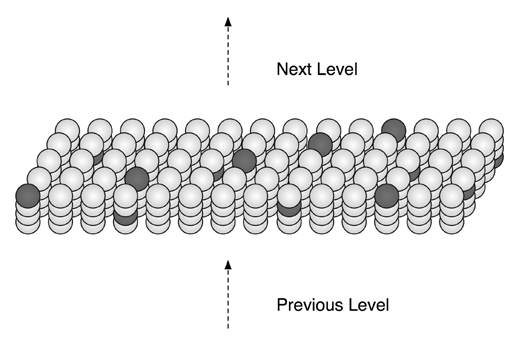
\includegraphics[width=0.95\textwidth]{region_sparse}}
    \only<3>{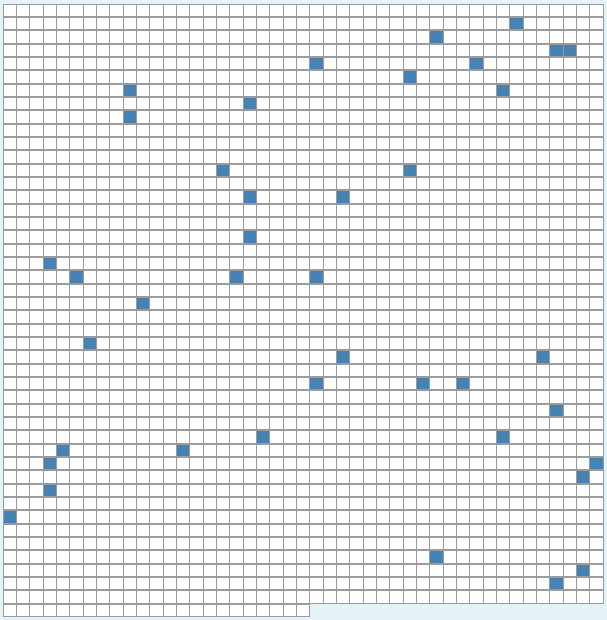
\includegraphics[height=0.9\textheight]{sdr_example}}
    % 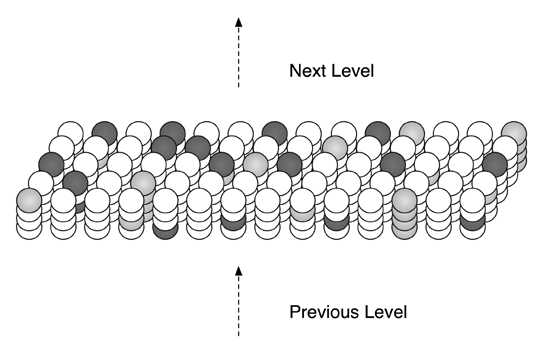
\includegraphics[width=0.9\textwidth]{region_predict}
\end{frame}


\begin{frame}[c]{Sparse Distributed Representation - Introduction}
    \Large
    \begin{itemize}[<+(1)->]
        \item Datastructure of the brain
        \item Sparse (around 2\% are active)
        \item Distributed (clusters are somewhat rare)
        \item Inhibitory Mechanisms
        \item Neuron states actually have 'meaning'
        \item Combined, they give context as well
        \item Many mechanisms in the brain would not work otherwise
    \end{itemize}
\end{frame}



% \subsection{Time}


\begin{frame}[c]{The role of Time}
    \Large
    Crucial for learning, inference and prediction.
    \begin{itemize}[<+(1)->]
        \item Inference is hard on static information
        \item Predictions are somewhat inherently time-based
        \item Learning is hard without feedback
    \end{itemize}
\end{frame}


